\documentclass[letterpaper]{article}
\usepackage{ms1report}
\usepackage[pdftex]{graphicx}
\usepackage{times}
\usepackage{helvet}
\usepackage{courier}
\usepackage[numbers]{natbib}
\pdfinfo{/Title (The Nature of Breath) /Author (Lauria Clarke)}

\title{The Nature of Breath: A Biomimetic Kinetic Sculpture That Breathes}
\author{Lauria Clarke\\ Parsons School of Design, The New School\\ New York, USA\\ clarl404@newschool.edu\\
\newline
\newline
}
\setcounter{secnumdepth}{0}

\begin{document} 
\maketitle

\begin{abstract}
The Nature of Breath is a kinetic sculpture exploring the sound and mechanics of human breath. By mimicking the mechanics of the human body this piece asks what it means for a machine to breath, drawing an uncertain line between what is considered natural and artificial. The Nature of Breath is also situated in response to the COVID-19 pandemic. In response to the virus' spread over the last two years, humans around the globe have become unusually attuned to the degrees of health or sickness that breath can indicate as well as the factors that may change one to the other. 
\end{abstract}

\keywords{Keywords}
kinetic sculpture, COVID-19, biomimicry, breath
%------------------------------
\section{Introduction}

% general introduction


Using the human act of breathing as a lens, this work attempts to lay a foundation for inquiry into the relationship between what is considered to be natural and what is or has been alive. While the focus of this work is on a specifically human form of breath, respiration in broader context is omnipresent in living organisms and is therefore an apt biological process with which to address this question. This machine may breath in a natural way, but its appearance clearly identifies it as something which is purely artificial.

% Respiration is an indicator of life at all scales - from single celled organisms to human beings. Whether involving oxygen in the conventional sense of breath, or operating at the cellular level, the process of energy production is essential to life as we know it. Taking breath, the most natural of human movements, into close consideration, this work examines the relationship between what is natural and what is, or has been, alive.

% With each human breath on this planet we move deeper into the anthropocene.

With the exception of cellular respiration, respiration in breathing organisms is a visibly mechanical process. Humans have created many mechanisms to mimic various aspects of the respiratory system for purposes ranging from medical devices, underwater exploration, to speech synthesis and more. Most of these devices are highly specialized and seek to mimic particular aspects of respiration such as oxygen delivery, or vocal modulation. These works rarely mimic the actual mechanics of the components of the human body responsible for respiration favoring more abstracted and efficient mechanical systems to achieve their goal. Using the freedom afforded by kinetic sculpture, this work attempts to blend a human-biomimetic approach -- highlighting the mechanical simplicity of the human body -- with a highly technical approach which allows for precise and complex control over the resulting breath.    

This work also asks us to consider the fragility of human breath in light of the COVID-19 pandemic. Seemingly overnight, much of the world became obsessed with breath as the toll of the virus spread. In the two years since, we have become incredibly attuned to the quality and sound of our own breath and what it may say about our mortality. This work seeks to probe these newfound sensitivities, forcing us to question which actions may lead breath to be easy or sharply painful. 


% Something about being alive. \cite{zimmer}


\subsection{Prior Work and Relevance}
% talk about the history of breathing apparatus and note that none mimic the human body
Mechanical ventilation has been around for a long time (include specific reference)...it  seeks to provide "replacement of the respiratory muscles". \cite{ventilatorhistory} This results in apparatuses that resemble the respiratory system only in the sense that they cause a regulated change in pressure which allows for oxygenation of the blood. The devices have no need, however, for recreating the process by which breath sounds are actually created. The field of biomimetic robotics has little use for such inquiry either -- respiration is not necessary for an electronic being and it is much easier to produce vocal noises digitally than mechanically. 

Two notable works in the field of kinetic sculpture provide some reference and context for this work, Maywa Denki's WAHHA GO GO and Rafael Lozano-Hemmer's Vicious Circular Breathing. \cite{denki} \cite{lozanohemmer} These two pieces provoke thought about breath, but still use simple bellow bases mechanisms to produce airflow. 

% context of the pandemic ventilators


\section{Implementation}

\subsection{System Breakdown}

While the avian respiratory system is, in fact, more complex, the human respiratory system is a very complicated biological system. \cite{gasexchangers} To simplify this system for translation to a constructable mechanical structure, I broke it down into three main sub-systems. Each sub-system exists solely for the purpose of generating breath noises and not for the actual exchange of oxygen as would normally occur during respiration.

\subsubsection{Actuation}

Actuation is the system which causes air to move through the respiratory system. In our own bodies this is achieved by the movement of the diaphragm. In ventilators this is often achieved by a pump or bellows.

\subsubsection{Storage}

Storage describes the way air is stored and contained during the act of breath. This is done by the lungs and is only necessary for the transfer of oxygen to the blood. While the lungs are arguably the most critical part of the respiratory system, they are the most difficult to simulate with accuracy and have relatively little bearing on the sound of breath in this context. 

\subsubsection{Modulation}

Modulation is the way the sound of breath is shaped as it leaves the body. This is achieved by the bronchial tree, trachea, larynx, and mouth. After actuation has been achieved, simulation of this system is the most relevant and interesting part of this.   

\subsection{Making and Testing}

So far a few different prototypes have been attempted. Focusing on the two main areas of inquiry, there have been auditory prototypes -- exploring the effect of disembodied breath noises -- as well as mechanical prototypes -- exploring ways to achieve a physiologically accurate breathing mechanism. In addition to creating a visual tie between the biological nature of the respiratory system, I chose to closely mimic the diaphragm and trachea in this way to prevent the noise of the mechanical components from overwhelming the noise of the breath produced. These approaches rely on material properties of -- elasticity and rigidity -- of latex and vinyl to be functional.

\subsubsection{Auditory Prototypes}

bucket experiement

p5 thing

\subsubsection{Physical Prototypes}

trachea

diaphragm

lever adjustment

\subsubsection{Final Prototypes}

the final result was a thing that nearly works and combines many of the elements from above

\section{Further Work}

well, there's always more to do...

the boris vian reference 


\section{Conclusion}

The complexity of the human respiratory system lies not in its gross mechanics, but in the materials and molecular mechanics that allow for the transfer of oxygen to the blood. The goal of this work was to isolate the mechanical components which form the noise created by breathing.  

bring this back to the question of the relationship between what is natural and what is alive

here is where I can cite some of the exciting reading I've done and talk about the big distinction of artificial and natural

\cite{zimmer}
\cite{haraway}
\cite{smith}




% why it's important to think about this in the context of humanity's relationship with the natural world


%\begin{figure}[h]
%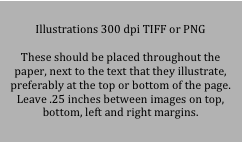
\includegraphics[width=3.31in]{figure.png}
%\caption{This is an example of figure caption. Note that all figures, and tables are to be referenced in the text. \copyright Respect Copyright.}
%\end{figure}
%
%\begin{figure*}
%
\includegraphics[width=\textwidth]{two-column-figure.png}
%\caption{Example of a double-column figure with caption. \copyright Respect Copyright.}
%\end{figure*}

\bibliographystyle{plain}
\bibliography{ms1report}

\section{Author Biography}
Lauria Clarke is an engineer and artist living in New York. She completed a MS in Computer Engineering at Northeastern University in 2017 and is currently pursuing an MFA in Design and Technology at The Parsons School of Design. She specializes in digital hardware design and kinetic sculpture and is always curious to learn more about humanity's relationship with the natural world.

% aspires to be a chocolate fish fisherman for Ben and Jerry's.

\section{Note to Harpreet}

Hi Harpreet, 

My apologies, this is quite rough. I plan to finish fleshing out the prior work and relevance section and then collect and polish all the writing I've done about my prototypes for the implementation section. I accidentally used up a lot of time writing about the uncanny valley and it's relevance in biomimetics/biodesign/biotechnology...which was far outside the scope of this paper

Lauria

\end{document}


% Masahiro Mori's 1970 essay prvided the framework for describing the confusing relationship between artifically created human-like robots and, as Mori calls us, real human beings. \cite{mori} This framework of thought has gained significant traction over the last 50 plus years as developments in technology have made it possiblt to mimic the human body with increasing accuracy. This definition has also been critical in the field of computer science as we consinute ot refine mahcine learning techniques which steadily approach the capacities of the uhman brain. This framework describes the point at which an artificial automaton approaches a point of being eeriely similar to a human being, creating a feeling of discomfort via the uncertainty of whether it is "real".

% For the lats fifty years this framework fo thought has been critical in describing technology's relationship with humanity. 

% Over the last *** years however, the fields of biodesign and bioart have increasingly been asking similar questions not about tchnology and humanity, but technology and nature. In light of the increasing environmental pressures of human imposed climate change, these questions are becoming increasingly urgent. Technology is now being used t oreplicate and mimic natural systems. As Donna Haraway noted in her paper, we must thin kbeyond the human. \cite{haraway} The capacity of our technology has surpassed the instinctually introspective and can now mimic what is natural outside of ourselves. This is a critical development and harkens back to mode indigenous ways of thinking - moving and working with natural systems, rather than in opposition to. 

% If our relationship with technology is extending beyond the human so to must our language. Mori's framework is distinctly human centric. How then do we apply this thinking to non-human natural world? Is Mori's valley merely a snaller depression within a much broader valley encompassing the whole of the natural world? Do humans deserve a place in that broader cintext? To frame this question more broadly, how do we, as human beings, distinguish between what is natural and what is atrificial? How is this distinction shifting as our techological capacity for the artifical increases at great cost to the natural world. 

%While its focus is on a specifically human foram of respiration, respiration in broader context is omnipresent in living organisms, thus providing a jumping off point for larger scope of inquiry into the relationship between what it means to be alive and what it means to be natural. Something about being alive. \cite{zimmer}
